\documentclass[jair, twoside,11pt,theapa]{article}
\usepackage{jair, theapa, rawfonts, amssymb}
\usepackage{graphicx}

\ShortHeadings{Performance of Retrieval with ASR transcribed queries}{Robinson}
\firstpageno{1}


\begin{document}
\title{Performance of Ad-hoc Retrieval with Automatic Speech Recognition Transcribed Queries}

\author{\name Max Robinson \email max.robinson@jhu.edu \\
       \addr Johns Hopkins University,\\
       Baltimore, MD 21218 USA
}

\maketitle

\begin{abstract}
\label{Abstract}
Ad-hoc retrieval with automatic speech recognition (ASR) transcribed queries presents a new set of challenges. The types of errors in transcribed queries are not the same as queries that were typed. This paper looks at the FIRE 2010 dataset with transcribed queries and investigates which simple indexing methods provide the most benefit to mitigate the errors that arise from ASR. The results showed that while the performance of ad-hoc retrieval is significantly degraded by poor transcription, using an indexing method of character 4-grams provided the best mitigation for errors introduced by ASR compared to character 3-grams and word indexing. 

\end{abstract}


\section{Introduction}
\label{Introduction}
Ad-hoc retrieval is a staple in modern day technology. With the world wide web and services such as Google and Microsoft's Bing, searching for relevant information has common practice. Now as technology has continued to advance, automatic speech recognition (ASR) is again at the forefront of technology through voice user interfaces for information retrieval. 

Much of where ASR is used today is to enable easier search for information. Many smart devices, including smart phones, have some sort of on board or built in ASR that is used for search. Everything from searching the Internet to looking up movies can have integration with ASR for these searches.

The goal of ASR is to have perfect accuracy in transcription of what a user says to what the system outputs as text. The ability accurately transcribe text in an every day scenario similar to a human has shown to be a difficult task. This provides an interesting problem to information retrieval systems to still provide relevant information even though the query could have errors. 

Providing accurate document retrieval with errors like spelling mistakes in queries is an active area of research. However, ASR transcribed text presents a new problem with the possibility of a transcribed word being entirely different than the intended word by the speaker. While, more accurate ASR would help fix this problem, it is not clear that all ASR will reach near perfect accuracy soon. 

This paper explores how different indexing methods for ad-hoc document retrieval affect the performance of retrieval using queries that are transcribed (trans) with ASR. To do so, this paper uses the English FIRE 2010 corpra (https://www.isical.ac.in/~clia/2010/) to test character 3-gram, 4-gram, and word based tokenization and indexing. For retrieval and executing queries, the open source search engine Elasticsearch is used. Mozilla's DeepSpeech implementation \cite{mozilla} was used to transcribe audio versions of the FIRE 2010 queries used for testing. 



\section{Previous Work and Background}
\label{Background}
Automatic speech recognition saw research into the domain with working systems as early as 1952 with a single speaker digit recognition system built by Bell Labs \cite{AsrHistory}. Since then, ASR has come a long ways. Services from companies like Google and Micrsoft are reaching close to 95\% accuracy \cite{Meeker} \cite{MS-human-accuracy}. Human accuracy is considered to be about 95\% \cite{MS-human-accuracy} as well, meaning that ASR is reaching a human level of accuracy very quickly. 

However, not all ASR is this accurate and not all uses of ASR can use tools provided by companies like Google or Microsoft. Alternative non-proprietary based solutions exist for this reason. A stand alone recurrent neural network called Deep Speech was developed by researchers at Baidu in 2014 \cite{Baidu-deep}. The network is an end-to-end network that tasks audio as input and outputs transcribed text. This was a break through in ASR by developing a single network that can do audio to text all by itself. 

The researchers claimed a 16\% error rate on a widely studied dataset, Switchboard Hub5'00. An open source implementation of Deep Speech by Mozilla \cite{mozilla} was later created with publicly available language models. This enables ASR without the need to use commercial services. 

%% Section on query error correction 
Errors in queries for information retrieval systems have also been studied. In a typical query system, errors in the query are typically caused by a human mistyping a word which results in a spelling mistake. Spelling mistakes have been studied for sometime and there are existing solutions such as edit distance, context sensitive spelling corrections, or phonetic corrections shown in books like Manning's ``Introduction to Information Retrieval" \cite{IntroductionIR}. 

Other techniques such as relevance feedback and query expansion have also been used to combat non-specific queries and enhance retrieval performance. Query expansion attempts to add relevant words to a query in the hopes that the expanded query provides better results. Relevance feedback aims to adjust a query based on the top documents initially retrieved to improve results. Relevance feedback can also be used as a corrective measure to suggest to a user a more likely query if a mistake was made. 


\section{Experiment}
\label{Experiment}
To test the affect of different indexing methods on retrieval performance for ASR transcribed queries the Forum for Information Retrieval Evaluation (FIRE) 2010 (https://www.isical.ac.\\in/\textasciitilde{}clia/2010/) English dataset was selected. The FIRE 2010 dataset is a collection of documents focused on news articles in the South Asia region. The documents are available in a few different languages, but for the purpose of this experiment the English version of these documents will be used. 

FIRE 2010 follows the TREC standard convention for document, topic, and qrels encodings. This allows the application of the standard TREC\_EVAL calculations and metrics to be used. The primary metric used in this experiment is the mean average precision (MAP) across the set of queries. The full TREC\_EVAL output for the experiment is available in Appendix C for reference. 

In order to test ASR transcription, the queries for FIRE 2010 had to be transformed into audio and then the audio must have ASR applied to it to obtain a transcribed query. To transform the queries, the queries were spoken out loud and recorded with an inexpensive headset microphone. The audio was recorded at 16KHz with 1 channel and a chunk size of 1024. 

Each recording was 20 seconds in length, even if speaking the query did not take 20 seconds. Queries were spoken with roughly the same cadence and speed to as much of a degree as possible by the speaker. The speaker was a native English speaker and words were spoken close to dictionary pronunciations typically (i.e. with little to no accent). The speaker was not familiar with many of the named entities in the query text so pronunciations of non-English words were done to the best of the speakers ability, following English phonetic rules. 

Mozilla's DeepSpeech implementation was chosen to transcribe the audio queries back to text. Mozilla's DeepSpeech was chosen because of its free availability and its popularity in the open source community. In addition, DeepSpeech is free and able to be run on a single computer with middling specifications. The model used for DeepSpeech is the freely available v0.3.0 model retrievable via the Mozilla DeepSpeech repository.

Elasticsearch (www.elastic.co) was used as the search engine and document storage. Elasticsearch is an open source and commercial search engine built on top of Apache Lucene (lucene.apache.org) which is an open source text search engine written in Java. Elasticsearch allows documents to be placed into different indexes and each index can specify a mapping, text analyzer, and tokenizer for indexing and querying on specific fields. 

Three indexes were created and used for the experiment. One index specified characters to be indexed using character 3-grams, another using character 4-grams, and the last used the standard Elasticsearch word indexing with stopword removal. For all indexes, text was translated into all lowercase characters prior to being indexed. An example of the Elasticsearch indexing settings can be seen in Appendix A. 

The documents for FIRE 2010 were indexed into Elasticsearch using a companion tool Logstash (www.elastic.co/products/logstash), after first being translated into tsv files. Logstash was used primarily to quickly index data into Elasticsearch. For each document, the entirety of the document was indexed, and the document ID was also stored with the document. 

Queries were made to Elasticsearch using both the transcribed queries and the original queries for comparison. The Elasticsearch query used was a standard Elasticsearch ``match" query. Elasticsearch preprocessed the query the same way it would index a document for the index being queried. It then executes a boolean ``or" query. The format of the query can be seen in Appendix B. Only the document ID was retrieved for each query and the score for each document was captured. 

In an attempt to retrieve as many relevant documents as possible for each query, the top 1000 documents were retrieved for each query. There were 50 queries total and the top 1000 documents were retrieved for each of those, resulting in a total of 50,000 documents retrieved across all queries. 

The results of each query were output in the standard TREC evaluation format for a trec\_top\_file. TREC\_EVAL was run on the results from executing all 50 transcribed queries against all indexes and executing all 50 original queries against all indexes. 


\section{Results and Analysis}
\label{Results}

ASR transcriptions are not without error. To understand how errors can impact querying the Word Error Rate (WER) was calculated for each query. Word error rate is a metric in ASR to try and measure how good the transcription is. It is similar to the Levenshtein distance for words, but rather uses words in a sentence rather than characters in a word. WER can be calculated by $WER = \frac{S + D + I}{N}$ where $S$ is the number of substitutions, $D$ is the number of deletions, $I$ is the number of inserts, and $N$ is the number of words in the reference. Lower is better. 

In addition the word recognition rate was also calculated. Word recognition rate is the number of matched words divided by the number of words in the reference sentence or document. Higher is better. The results were then averaged to determine an average word error rate across all queries. Both WER and WRR were calculated using a open source third-party python library, asr-evalutation (https://github.com/belambert/asr-evaluation).

\begin{table}[h!]
    \caption{Word Error Rate and Word Recognition Rage Per Query}
    \label{Table1}
    \begin{minipage}{.5\linewidth}
        \centering
        \begin{tabular}{|l|l|l|}
        \hline
        Query ID & WER \%    & WRR \%    \\ \hline
        76       & 55      & 55      \\ \hline
        77       & 91.667  & 25      \\ \hline
        78       & 103.704 & 44.444  \\ \hline
        79       & 62.5    & 50      \\ \hline
        80       & 80      & 45      \\ \hline
        81       & 55.556  & 55.556  \\ \hline
        82       & 85.714  & 57.143  \\ \hline
        83       & 120.833 & 29.167  \\ \hline
        84       & 72.222  & 50      \\ \hline
        85       & 78.571  & 28.571  \\ \hline
        86       & 62.5    & 54.167  \\ \hline
        87       & 87.097  & 19.355  \\ \hline
        88       & 68.571  & 31.429  \\ \hline
        89       & 92.308  & 38.462  \\ \hline
        90       & 70.833  & 50      \\ \hline
        91       & 84.615  & 46.154  \\ \hline
        92       & 75      & 25      \\ \hline
        93       & 40      & 70      \\ \hline
        94       & 47.368  & 63.158  \\ \hline
        95       & 63.158  & 52.632  \\ \hline
        96       & 100     & 23.077  \\ \hline
        97       & 66.667  & 47.619  \\ \hline
        98       & 92.857  & 42.857  \\ \hline
        99       & 106.667 & 33.333  \\ \hline
        100      & 85.714  & 42.857  \\ \hline
        \end{tabular}
    \end{minipage}%
    \begin{minipage}{.5\linewidth} 
        \centering
        \begin{tabular}{|l|l|l|}
        \hline
        Query ID & WER \%    & WRR \%    \\ \hline
        101      & 77.778  & 48.148  \\ \hline
        102      & 86.667  & 53.333  \\ \hline
        103      & 100     & 47.368  \\ \hline
        104      & 95.833  & 37.5    \\ \hline
        105      & 68      & 52      \\ \hline
        106      & 93.33   & 6.667   \\ \hline
        107      & 89.474  & 52.632  \\ \hline
        108      & 89.474  & 36.842  \\ \hline
        109      & 43.478  & 65.217  \\ \hline
        110      & 107.143 & 42.857  \\ \hline
        111      & 66.667  & 53.333  \\ \hline
        112      & 94.118  & 41.176  \\ \hline
        113      & 56.25   & 62.5    \\ \hline
        114      & 67.857  & 53.571  \\ \hline
        115      & 116.667 & 41.667  \\ \hline
        116      & 88.235  & 47.059  \\ \hline
        117      & 50      & 67.857  \\ \hline
        118      & 94.444  & 44.4444 \\ \hline
        119      & 100     & 0       \\ \hline
        120      & 86.207  & 13.793  \\ \hline
        121      & 144.44  & 33.333  \\ \hline
        122      & 100     & 35.714  \\ \hline
        123      & 111.111 & 22.222  \\ \hline
        124      & 50      & 62.5    \\ \hline
        125      & 85.714  & 42.857  \\ \hline
        \end{tabular}
    \end{minipage}
\end{table}

\begin{table}
    \centering
    \caption{Aggregated WER and WRR percentages}
    \label{Table2}
    \begin{tabular}{|l|l|l|l|}
        \hline
                  & Average \%    & Min \%    & Max \%    \\ \hline
        WER       & 82.24       &  40     & 144.44  \\ \hline
        WRR       & 42.891428   & 0       & 70      \\ \hline
    \end{tabular}
\end{table}

Table \ref{Table1} shows the WER and WRR for each query. Table \ref{Table2} shows some aggregated statistics about the WER and WRR. In general, the WER was very high for all queries. Some queries even had WERs that were above 100\%. This means is that the transcribed text required more edits ans substitutions than words in the original query. The best WER achieved was about 40\%, which is still a ways off of 16\% error rate claimed by Baidu researchers. 

Investigating the translated queries leads to a hypothesis for the poor ASR performance. While the FIRE 2010 dataset is a set of English language documents and queries, many of the named entities in the queries are not English words. However, the model used for DeepSpeech was an English model. These non-English words might not have been covered by the training or test set for the model. This could cause many errors in query translation. 

\begin{figure}
    \centering
    \caption{Ground Truth and Hypothesized Queries from DeepSpeech}
    \label{query_Transcribe_fail}
    \fbox{%
    \begin{minipage}{\textwidth}
        Q77 GT: \textit{Attacks by Hezbollah guerrillas Attacks by Hezbollah guerrillas on Indian and Israeli forces.} \\
        Q77 Transcribed: \textit{attack by has below garillas attacked by hasbelocarillos on indian and is rally forcees} \\

        Q121 GT: \textit{Blasts on Samjhauta Express Deadly explosions on the Samjhauta Express.}\\
        Q121 Transcribed: \textit{blasts on some shot to it press that ly explosions on these seven shot a expresss}
      \end{minipage}
    }
\end{figure}

Figure \ref{query_Transcribe_fail} shows two example ground truth queries from FIRE 2010 and the counter part transcription from DeepSpeech. In Q77, ``Hezbollah" can be seen to cause a failure in transcription just for that word, and thus loosing the named entity in the sentence. Q121, the word ``Samjhauta" appears to cause a failure in transcription but not only for the single word. In this case, many following words seem to be effected by this mistake in transcription. 

In addition to non-English words in the queries, the speaker who was recorded was also unfamiliar with the pronunciation of many of these non-English words. The resulting audio for these words could be poor as the pronunciation could be incorrect which could lead to possibly worse results. The audio quality for query transcription could also have played a factor as additional noise from the mic or background could have played a role. The audio recording setup was not dislike many setups for a consumer, so the audio quality should be at least partially representative of a real world circumstance.  

The effect ASR error had on query results was substantial. Figure \ref{fig:MAP_all} shows the MAP for queries using transcribed queries versus the ground truth queries across all indexing methods; 3-grams, 4-grams, and words. It can be seen that transcribed queries did significantly worse than their ground truth counter parts for all indexing methods.


\begin{figure}[h!]
\centering
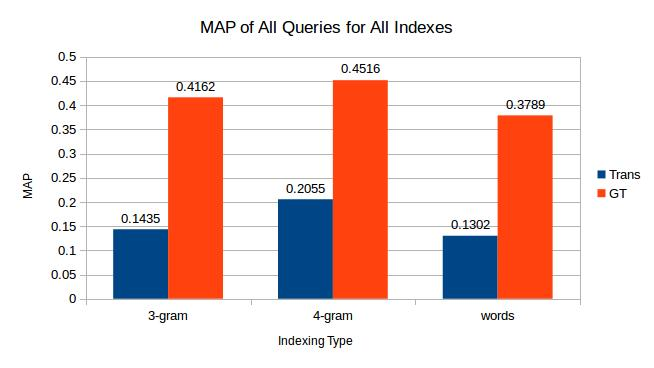
\includegraphics[width=1.0\linewidth]{../ResultImages/MAP}
\vspace{-3em}
\caption{MAP of Ground Truth and Transcribed Queries for All Indexing Schemes}
\label{fig:MAP_all}
\end{figure}


\begin{table}[]
\centering
\caption{\% of Ground Truth MAP per Indexing Type}
\label{MAP_mitigation}
\begin{tabular}{|l|l|l|l|}
\hline
Indexing & Trans  & GT     & \% of GT performance      \\ \hline
3-gram    & 0.1435 & 0.4162 & 34.47861605 \\ \hline
4-gram    & 0.2055 & 0.4516 & 45.50487157 \\ \hline
words    & 0.1302 & 0.3789 & 34.36262866 \\ \hline
\end{tabular}
\end{table}

Overall, 4-gram indexing had the best MAP both for the ground truth queries and for transcribed queries. This provides additional evidence to previous works that showed that 4-grams are particularly effective, especially for European languages \cite{McNamee2004}. In addition, previous work showed that 4-grams are the most effective for the Hindi FIRE 2010 dataset \cite{Vishwakarma}. This seems to be the case for the English FIRE 2010 dataset. 

While the performance of 4-grams has been shown before, the interesting part for this experiment is how 4-grams were able to reduce the impact that ASR error had on query performance. Table \ref{MAP_mitigation} shows the percentage of performance the transcribed query had compared to its ground truth counter. The transcribed queries using 3-grams performed only 34\% as well when compared to ground truth queries using 3-grams. So transcription decreased MAP by about 66\% for 3-grams. The same is true for words, about a 66\% reduction in performance. 

For 4-grams, only had about a 55\% reduction in performance compared to its ground truth counter parts. This shows that 4-grams were more effective at reducing the effect of ASR error on retrieval than 3-grams and words. 

\begin{figure}
\centering
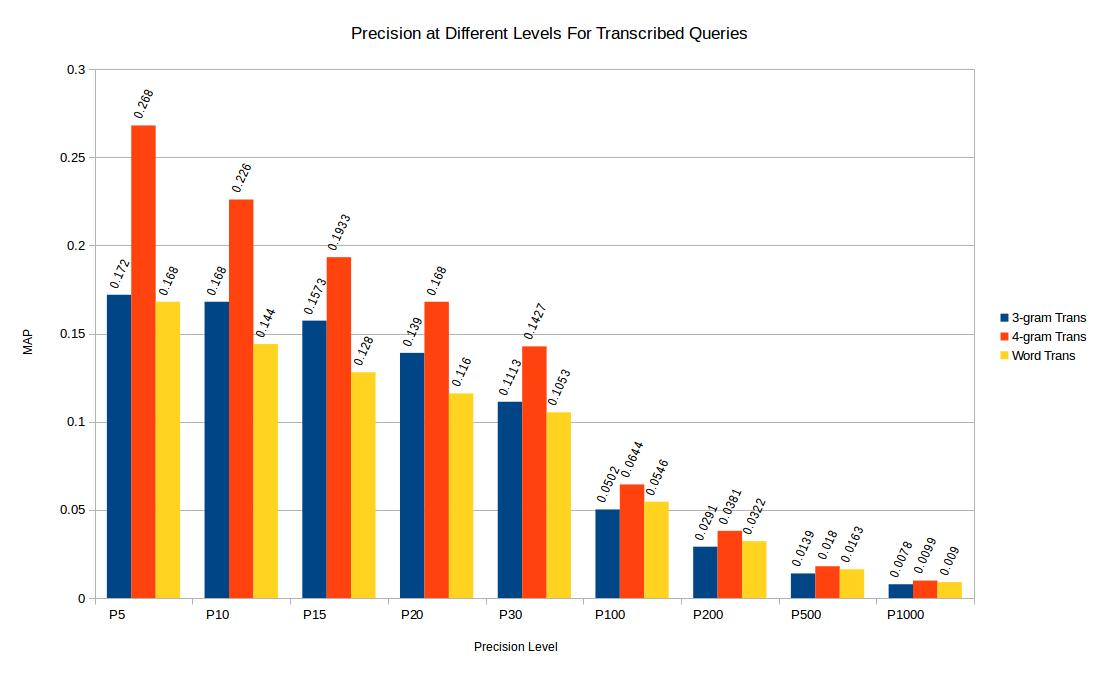
\includegraphics[width=1.0\linewidth]{../ResultImages/Precisions}
\caption{Precision at different Levels for Transcribed Queries}
\label{fig:Precisions}
\end{figure}

The performance of 4-grams can also be seen when comparing precision with different numbers of documents retrieved. Figure \ref{fig:Precisions} shows precision for the number of documents retrieved. 4-grams can be seen to have much higher precision compared to 3-grams and words especially when fewer documents are retrieved. This indicates that 4-grams would also perform better if only looking at the top 30 or so documents. 

It is slightly surprising that character 3-grams and word indexing had such similar performance. The motivation behind 3-grams was to index possible like character sequences that might exist if whole word were incorrectly substituted in the transcribed query. However, it appears that 3-grams were not able to pick up enough extra information to perform much better than word indexing. This is most likely because the words substituted were not as similar in short character sequences as originally thought. Like in Figure \ref{query_Transcribe_fail}, ``Hezbollah" is transcribed to ``hasbelocarillos" where the character 3-gram ``has" instead of ``hez" which might hurt retrieval more than help in this case. 

For this particular dataset and transcriptions, the hypothesis is that the character 4-gram indexing was able to capture larger overlapping segments of partially correct words in the ASR transcription. In Figure \ref{query_Transcribe_fail}, Q77 a 4-gram that would have been captured includes ``by h". This 4-gram contains an important piece of information about the following named entity ``Hezbollah". The named entity in the transcribed query is incorrect but this 4-gram exists in both queries and might be enough to narrow the search. The 4-gram ``rill" later in the sentence that should belong to ``guerrillas" is also in both queries, and is likely to belong to fewer words than other sequences. 

These character 4-grams, while still capturing errors, appear to be able to capture enough identifying characteristics in the queries to be more effective. These parts of named entities that might be captured, could be one of the reasons that 4-grams performed better than the other indexing methods. 


\section{Future Work}
\label{Future}
While this paper explored some aspects of ASR integration with ad-hoc retrieval there is much more work that could be done. The DeepSpeech off the shelf model for ASR seems to need a different dataset for queries if the effects of ASR with document retrieval are to be inspected with a lower average word error rate. The high word error rate provided good contrast for this paper, but more realistic performance might be achieved by using a dataset consisting of common English words to transcribe. 

More work can also be done to analyze where ASR makes mistakes and how other forms of tokenization and indexing can possibly reconcile these errors. Stemming for transcriptions would be an area of future work to possibly avoid plural or past tense errors. Soundex type indexing might be tried in order to capture the sounds of transcribed words that might account for errors. 

\section{Conclusion}
\label{Conclusion}
In this paper, the overlap between automatic speech recognition and ad-hoc retrieval was explored. The interesting problem of errors through transcriptions motivated a look at what basic tokenizing and indexing techniques could be applied to mitigate these errors. While the ASR used for the experiments had high word error rates for transcribed queries, it magnified the differences between the different indexing approaches. 

The results of the experiment showed that character 4-grams where the best indexing choice to mitigate error introduced by transcribing queries using Mozilla's DeepSpeech implementation. Not only did 4-grams mitigate error best overall, it also provided the best performance when looking at only the top few documents returned. 

While more work can be done to explore additional techniques to mitigate error from ASR, this work reaffirms that character 4-grams perform well in document retrieval and are good starting place for ASR transcription error mitigation for document retrieval. 



\vskip 0.2in
\bibliography{ProjectWriteup}
\bibliographystyle{theapa}

\raggedbottom
\pagebreak 

\section*{Appendix A: Elasticsearch Index 4-gram Configuration}
\begin{verbatim}
{
  "settings":{
    "number_of_shards" :   1,
    "number_of_replicas" : 0,
    "analysis":{
      "analyzer":{
        "4gram":{ 
           "type":"custom",
           "tokenizer":"4grams",
           "filter":[
              "lowercase"
           ]
        }
       },
      "tokenizer": {
        "4grams": {
          "type": "ngram",
          "min_gram": 4,
          "max_gram": 4,
          "token_chars": []
        }
      }
    }
  },
  "mappings": {
    "doc": {
      "properties": {
        "doc": { 
          "type": "text",
          "analyzer":"4gram",
          "search_analyzer":"4gram"
        }
      }
    }
  }
}
\end{verbatim}

\pagebreak

\section*{Appendix B: Elasticsearch Query}
\label{Appendix B}
\begin{verbatim}
{
    "_source": ["docID"],
    "query": {
        "match": {
            "doc": "<query text>"
        }
    },
    "size": 1000
}
\end{verbatim}

\pagebreak
\section*{Appendix C: Full TREC\_EVAL output} 
\begin{table}[h!]
\begin{tabular}{|l|l|l|l|l|l|l|}
\hline
               & 3-grams trans & 3-grams gt & 4-grams trans & 4-grams gt & words trans & words gt \\ \hline
num\_q         & 50        & 50       & 50        & 50        & 50        & 50       \\ \hline
num\_ret       & 50000     & 50000    & 50000     & 50000     & 50000     & 50000    \\ \hline
num\_rel       & 653       & 653      & 653       & 653       & 653       & 653      \\ \hline
num\_rel\_ret  & 392       & 640      & 497       & 650       & 449       & 635      \\ \hline
map            & 0.1435    & 0.4162   & 0.2055    & 0.4516    & 0.1302    & 0.3789   \\ \hline
gm\_ap         & 0.0175    & 0.3017   & 0.0583    & 0.339     & 0.0212    & 0.2496   \\ \hline
R-prec         & 0.1581    & 0.3913   & 0.2143    & 0.4172    & 0.1316    & 0.3553   \\ \hline
bpref          & 0.5646    & 0.9785   & 0.7407    & 0.9973    & 0.6417    & 0.9665   \\ \hline
recip\_rank    & 0.3471    & 0.6968   & 0.4959    & 0.735     & 0.2818    & 0.676    \\ \hline
ircl\_prn.0.00 & 0.3553    & 0.7339   & 0.5168    & 0.7625    & 0.3048    & 0.7134   \\ \hline
ircl\_prn.0.10 & 0.2906    & 0.6998   & 0.4051    & 0.6912    & 0.241     & 0.6264   \\ \hline
ircl\_prn.0.20 & 0.2584    & 0.5787   & 0.3192    & 0.6113    & 0.209     & 0.5316   \\ \hline
ircl\_prn.0.30 & 0.1776    & 0.5185   & 0.2624    & 0.5544    & 0.1641    & 0.4538   \\ \hline
ircl\_prn.0.40 & 0.1552    & 0.4633   & 0.2393    & 0.5165    & 0.1461    & 0.4055   \\ \hline
ircl\_prn.0.50 & 0.1313    & 0.4093   & 0.2095    & 0.4607    & 0.1272    & 0.3715   \\ \hline
ircl\_prn.0.60 & 0.1088    & 0.3786   & 0.1533    & 0.4267    & 0.1109    & 0.3432   \\ \hline
ircl\_prn.0.70 & 0.0788    & 0.3208   & 0.1245    & 0.3655    & 0.0885    & 0.3264   \\ \hline
ircl\_prn.0.80 & 0.0565    & 0.2797   & 0.1025    & 0.3276    & 0.0778    & 0.2741   \\ \hline
ircl\_prn.0.90 & 0.041     & 0.2256   & 0.0708    & 0.2508    & 0.0505    & 0.2061   \\ \hline
ircl\_prn.1.00 & 0.0359    & 0.1957   & 0.0483    & 0.206     & 0.0316    & 0.1592   \\ \hline
P5             & 0.172     & 0.508    & 0.268     & 0.536     & 0.168     & 0.412    \\ \hline
P10            & 0.168     & 0.38     & 0.226     & 0.408     & 0.144     & 0.338    \\ \hline
P15            & 0.1573    & 0.336    & 0.1933    & 0.3573    & 0.128     & 0.3067   \\ \hline
P20            & 0.139     & 0.297    & 0.168     & 0.318     & 0.116     & 0.267    \\ \hline
P30            & 0.1113    & 0.2467   & 0.1427    & 0.2513    & 0.1053    & 0.2213   \\ \hline
P100           & 0.0502    & 0.1096   & 0.0644    & 0.1164    & 0.0546    & 0.1052   \\ \hline
P200           & 0.0291    & 0.0608   & 0.0381    & 0.0623    & 0.0322    & 0.0574   \\ \hline
P500           & 0.0139    & 0.0252   & 0.018     & 0.0257    & 0.0163    & 0.0247   \\ \hline
P1000          & 0.0078    & 0.0128   & 0.0099    & 0.013     & 0.009     & 0.0127   \\ \hline
\end{tabular}
\end{table}

\end{document}
